\documentclass{article}

\usepackage{amsmath}
\usepackage{amssymb}
\usepackage{bm}
\usepackage{color}
\usepackage{CJKutf8}
\usepackage{color}
\usepackage{enumitem}
\usepackage{graphicx}
\usepackage{indentfirst}
\usepackage{listings}
\usepackage{mathdots}
\usepackage{tikz}
\usepackage{wasysym}
\usepackage{xcolor}

\setlength{\parindent}{2em}

\usetikzlibrary{shapes,arrows, automata}

\allowdisplaybreaks

\newcommand{\hytt}[1]{\texttt{\hyphenchar\font=\defaulthyphenchar #1}}
\hyphenation{read-Sym-bol re-ad-Space-Tab-New-line str-Tab}

\definecolor{mygreen}{rgb}{0,0.6,0}
\definecolor{mygray}{rgb}{0.5,0.5,0.5}
\definecolor{mymauve}{rgb}{0.58,0,0.82}
%\footnotesize
\lstset{ %
  backgroundcolor=\color{white},   % choose the background color; you must add \usepackage{color} or \usepackage{xcolor}
  basicstyle=\ttfamily,            % the size of the fonts that are used for the code
  breakatwhitespace=false,         % sets if automatic breaks should only happen at whitespace
  breaklines=true,                 % sets automatic line breaking
  captionpos=b,                    % sets the caption-position to bottom
  commentstyle=\ttfamily\color{mygreen},    
                                   % comment style
  deletekeywords={},               % if you want to delete keywords from the given language
  escapeinside={},                 % if you want to add LaTeX within your code
  extendedchars=true,              % lets you use non-ASCII characters; for 8-bits encodings only, does not work with UTF-8
  frame=single,                    % adds a frame around the code
  keepspaces=true,                 % keeps spaces in text, useful for keeping indentation of code (possibly needs columns=flexible)
  keywordstyle=\color{blue},       % keyword style
  language=VHDL,                    % the language of the code
  morekeywords={},                 % if you want to add more keywords to the set
  numbers=left,                    % where to put the line-numbers; possible values are (none, left, right)
  numbersep=5pt,                   % how far the line-numbers are from the code
  numberstyle=\tiny\color{mygray}, % the style that is used for the line-numbers
  rulecolor=\color{black},         % if not set, the frame-color may be changed on line-breaks within not-black text (e.g. comments (green here))
  showspaces=false,                % show spaces everywhere adding particular underscores; it overrides 'showstringspaces'
  showstringspaces=false,          % underline spaces within strings only
  showtabs=false,                  % show tabs within strings adding particular underscores
  stepnumber=1,                    % the step between two line-numbers. If it's 1, each line will be numbered
  stringstyle=\color{mymauve},     % string literal style
  tabsize=2,                       % sets default tabsize to 2 spaces
  title=\lstname                   % show the filename of files included with \lstinputlisting; also try caption instead of title
}

\begin{document}
\begin{CJK*}{UTF8}{gbsn}
\CJKtilde

\title{实验二(1) 计数器设计实验}

\author{计算机1202 张艺瀚\\学号:20123852}
\maketitle

\section{实验目的}
\begin{enumerate}
\item 学习计数器不同设计方法。
\item 学习掌握VHDL中不同输出类型在具体应用时的区别(OUT、INOUT、BUFFER)。
\item 学习掌握时序电路仿真方法。
\end{enumerate}

\section{实验内容}
\begin{enumerate}
\item 采用VHDL设计方法,设计一个60进制计数器,采用BCD码输出。
\item 给出上述设计的仿真结果。
\end{enumerate}

\section{实验设备}
\begin{enumerate}
\item 清华同方PⅣ 2.4G/256M60G
\item ISE 6.2i—Windows软件系统
\end{enumerate}

%\section{实验步骤}

\section{实验程序}
\begin{center}
\begin{lstlisting}[caption = {60进制计数器代码清单}, label = {lst: counterlst}]
library IEEE;
use IEEE.STD_LOGIC_1164.ALL;
use IEEE.STD_LOGIC_ARITH.ALL;
use IEEE.STD_LOGIC_UNSIGNED.ALL;

--  Uncomment the following lines to use the declarations that are
--  provided for instantiating Xilinx primitive components.
--library UNISIM;
--use UNISIM.VComponents.all;

entity c is port(
	clk, en, clr: in std_logic;
	qh, ql: out std_logic_vector(3 downto 0));
end c;

architecture Behavioral of c is

signal qccl: std_logic;
signal qtempl, qtemph: std_logic_vector(3 downto 0);

begin

ql<=qtempl;
qccl<=qtempl(3) and not qtempl(2) and not qtempl(1) and qtempl(0);
qh<=qtemph;

p1: process(clk, en, clr)
begin
	if clr='1' then
		qtempl<="0000";
	else
		if rising_edge(clk) then
			if en='1' then
				if qtempl="1001" then
					qtempl<="0000";
				else
					qtempl<=qtempl+'1';
				end if;
			end if;
		end if;
	end if;
end process p1;

p2: process(clk, clr)
begin
	if clr='1' then
		qtemph<="0000";
	else
		if rising_edge(clk) then
			if qccl='1' then
				if qtemph="0101" then
					qtemph<="0000";
				else
					qtemph<=qtemph+'1';
				end if;
			end if;
		end if;
	end if;
end process p2;

end Behavioral;
\end{lstlisting}
\end{center}

\section{仿真结果}
\begin{center}
\begin{figure}[h!]
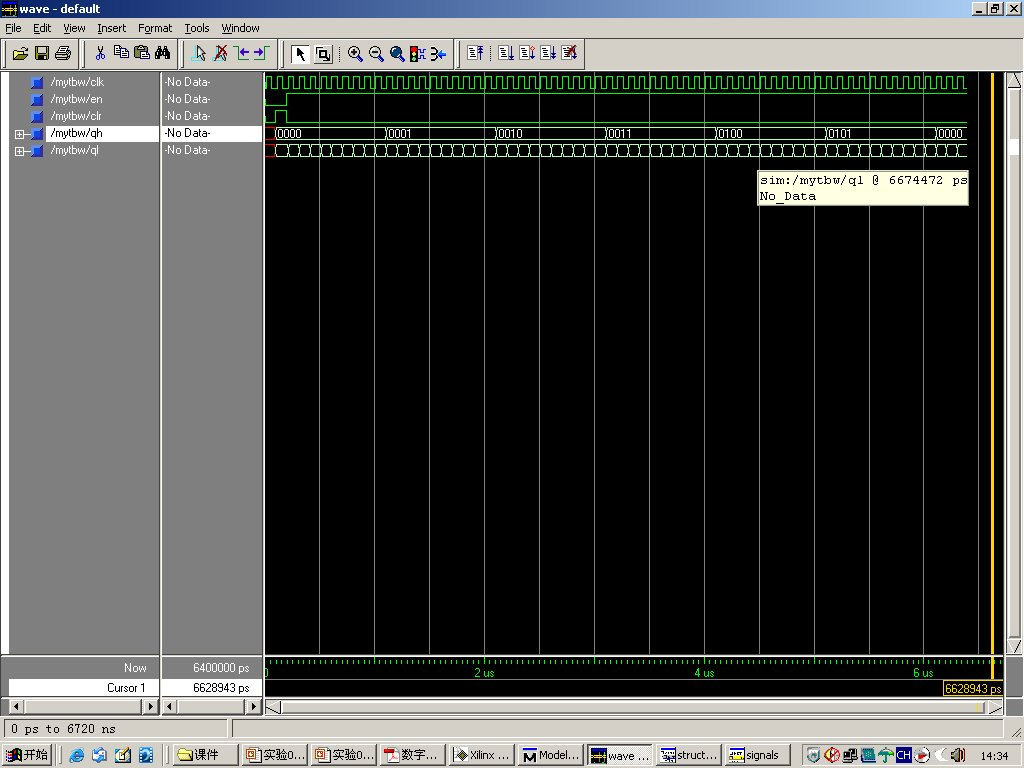
\includegraphics[width=\textwidth]{counter.jpg}
\caption{60进制计数器仿真波形图}
\label{fig: cfig}
\end{figure}
\end{center}

\end{CJK*}
\end{document}
